\documentclass{subfiles}

\begin{document}

  \chapter{Diseño y modelado en 3D}
  \label{chap:4}

    Para diseñar los dos modelos tridimensionales con los que contamos, tuvimos que hacer una pequeña investigación sobre herramientas de diseño y modelado en 3D, ya que nuestra empresa no está especializada en este tipo de trabajos. Además, nuestro equipo de Marketing no podía ocuparse de estos desarrollos debido a que solo trabaja con diseños bidimensionales y a que el tiempo necesario a invertir en formaciones y en el propio modelado era considerablemente alto, por lo que no pudimos contar con su ayuda. La mayor parte de las webs que hacen comparaciones entre distintas herramientas de diseño y modelado 3D mostraban las mismas herramientas, que son las que barajamos en un principio: \blender \cite{web:blender}, \unreal \cite{web:unreal} y \unity \cite{web:unity}.

    \begin{itemize}
        \item \textbf{\blender} es una de las herramientas más famosas que existen hoy en día para diseño de modelos 3D por su potencial y por ser gratuita. Se trata de una aplicación de código libre muy extendida que dispone también de un manual de uso y tutorial \cite{web:blender_manual} a disposición de todos los usuarios, además de una de las comunidades más grandes para resolución de dudas. Sus funcionalidades cubrían todas nuestras necesidades (modelado, animación, creación...), aunque la interfaz no es considerada de las mejores.
        
        \item \textbf{\unreal} era otra de nuestras opciones, debido a que cuenta con una gran trayectoria tanto en series y películas de animación como en videojuegos, aunque también se utiliza en ocasiones para arquitectura y diseño. Esta aplicación es una de las más potentes del mercado y cuenta además con cursos online, documentación y tutoriales \cite{web:unreal_learn}, así como foros para consulta de dudas \cite{web:unreal_forum}. Esta aplicación tiene como gran desventaja que la cantidad de funcionalidades al estar adaptado a esta gran variedad de usos hace de ella que sea más compleja de utilizar. Además, para poder exportar los modelos en el formato que necesitamos (\gltf o \glb), requeríamos de un plugin a mayores \cite{web:unreal_plugin}.
        
        \item Por último, habíamos barajado también la posibilidad de utilizar \textbf{\unity}, una herramienta inicialmente creada para diseño de videojuegos, pero que también cubre todas las necesidades de modelado y animación que necesitábamos. Esta aplicación es algo menos potente que la anterior opción, pero también es una de las herramientas más utilizadas del mercado, pudiendo darnos una solución más que aceptable. \unity también requiere de una extensión para poder exportar modelos a \glb o a \gltf \cite{web:unity_plugin}.
    \end{itemize}

    \paragraph{}
    Finalmente, de entre las distintas herramientas, nos decantamos por \blender, siendo una de las principales razones la económica: la libertad de uso de \blender está definida por una licencia \textit{GNU General Public License} \cite{web:blender_license,web:gnulicense}, por lo que no tendríamos ningún problema al utilizarlo como empresa. Las otras dos herramientas, al contrario, requieren de licencias si se van a utilizar en entornos profesionales \cite{web:unity_pricing,web:unreal_licensing}, por lo que podría suponernos un gasto a mayores para una diferencia que, por nuestra baja experiencia en esta materia, no sabríamos encontrar. Además, encontramos a un compañero en nuestra empresa que había usado \blender anteriormente para crear pequeños videojuegos a modo de afición y que podía aconsejarnos y ayudarnos a la hora de usar dicha herramienta, punto que sería definitivo a la hora de tomar la decisión.

    \paragraph{}
    Una vez decidimos la herramienta a utilizar, contemplamos también la idea de utilizar una aplicación a mayores que estuviese especializada en generar figuras humanas desde cero, debido a que su creación a través de las herramientas anteriormente expuestas es muy costosa y requiere de personal más experimentado para obtener unos resultados que nos pareciesen aceptables para el proyecto.
    
    \paragraph{}
    Inicialmente, optamos por buscar herramientas que generasen modelos 3D a partir de múltiples fotografías de una misma persona desde distintos ángulos: aplicaciones como \textit{Meshroom} \cite{web:meshroom} están orientadas a generar, no solo figuras humanas, sino también elementos del entorno como árboles, estatuas, edificios, etc. mediante fotogrametría, concepto que ellos mismos definen como la ciencia de tomar medidas a partir de fotografías.

    \paragraph{}
    También valoramos la posibilidad de utilizar un banco de modelos 3D previamente generados y que pudiéramos modificar a nuestro placer, como lo que ofrece \textit{Renderpeople} \cite{web:renderpeople}. Esto, en combinación con \blender, nos permitiría modificar los aspectos necesarios del modelo y ahorrarnos un costoso trabajo de generación desde cero.

    \paragraph{}
    Sin embargo, y también bajo recomendación del mismo compañero antes mencionado, finalmente nos decantamos por usar la aplicación \makehuman \cite{web:makehuman}: una herramienta de código abierto y libre uso orientado a la generación de modelos 3D humanoides que permite un amplísimo abanico de características a personalizar en estos: desde aspectos básicos como su altura hasta detalles minúsculos como el tamaño del lóbulo de la oreja. Todo esto, además, lo ofrece mediante una interfaz completamente sencilla de utilizar, a lo que además hay que sumar que permite utilizar, también de manera sencilla, texturas personalizadas para el personaje, por lo que podríamos dotarlo de elementos que pudiéramos hacer completamente nuestros.

    \paragraph{}
    Uniendo todo esto, podemos comenzar con el trabajo de modelado.

    \section{Creación mediante \makehuman}
    \label{sec:4.1}

    La herramienta \makehuman nos ofrece, desde un inicio, una serie de pestañas que nos van informando de qué conjuntos de características podemos modificar. Para el desarrollo de este modelo, nos vamos a centrar en solo algunas de estas pestañas. La aplicación ofrece las siguientes opciones:

    \begin{itemize}
        \item \textbf{Modelado}: para definir las proporciones y características de la figura humana del modelo.
        \item \textbf{Geometrías}: para modificar la forma de algunas de las estructuras del modelo, como dentadura, ojos, ropa, pelo, etc.
        \item \textbf{Materiales}: para modificar las texturas de las que estarán formadas las mallas que componen la figura.
        \item \textbf{Pose/Animación}: para establecer las opciones relacionadas con estas, como el esqueleto o la posición en la que reposa la figura.
    \end{itemize}

    \begin{figure}
    \centering
    \fbox{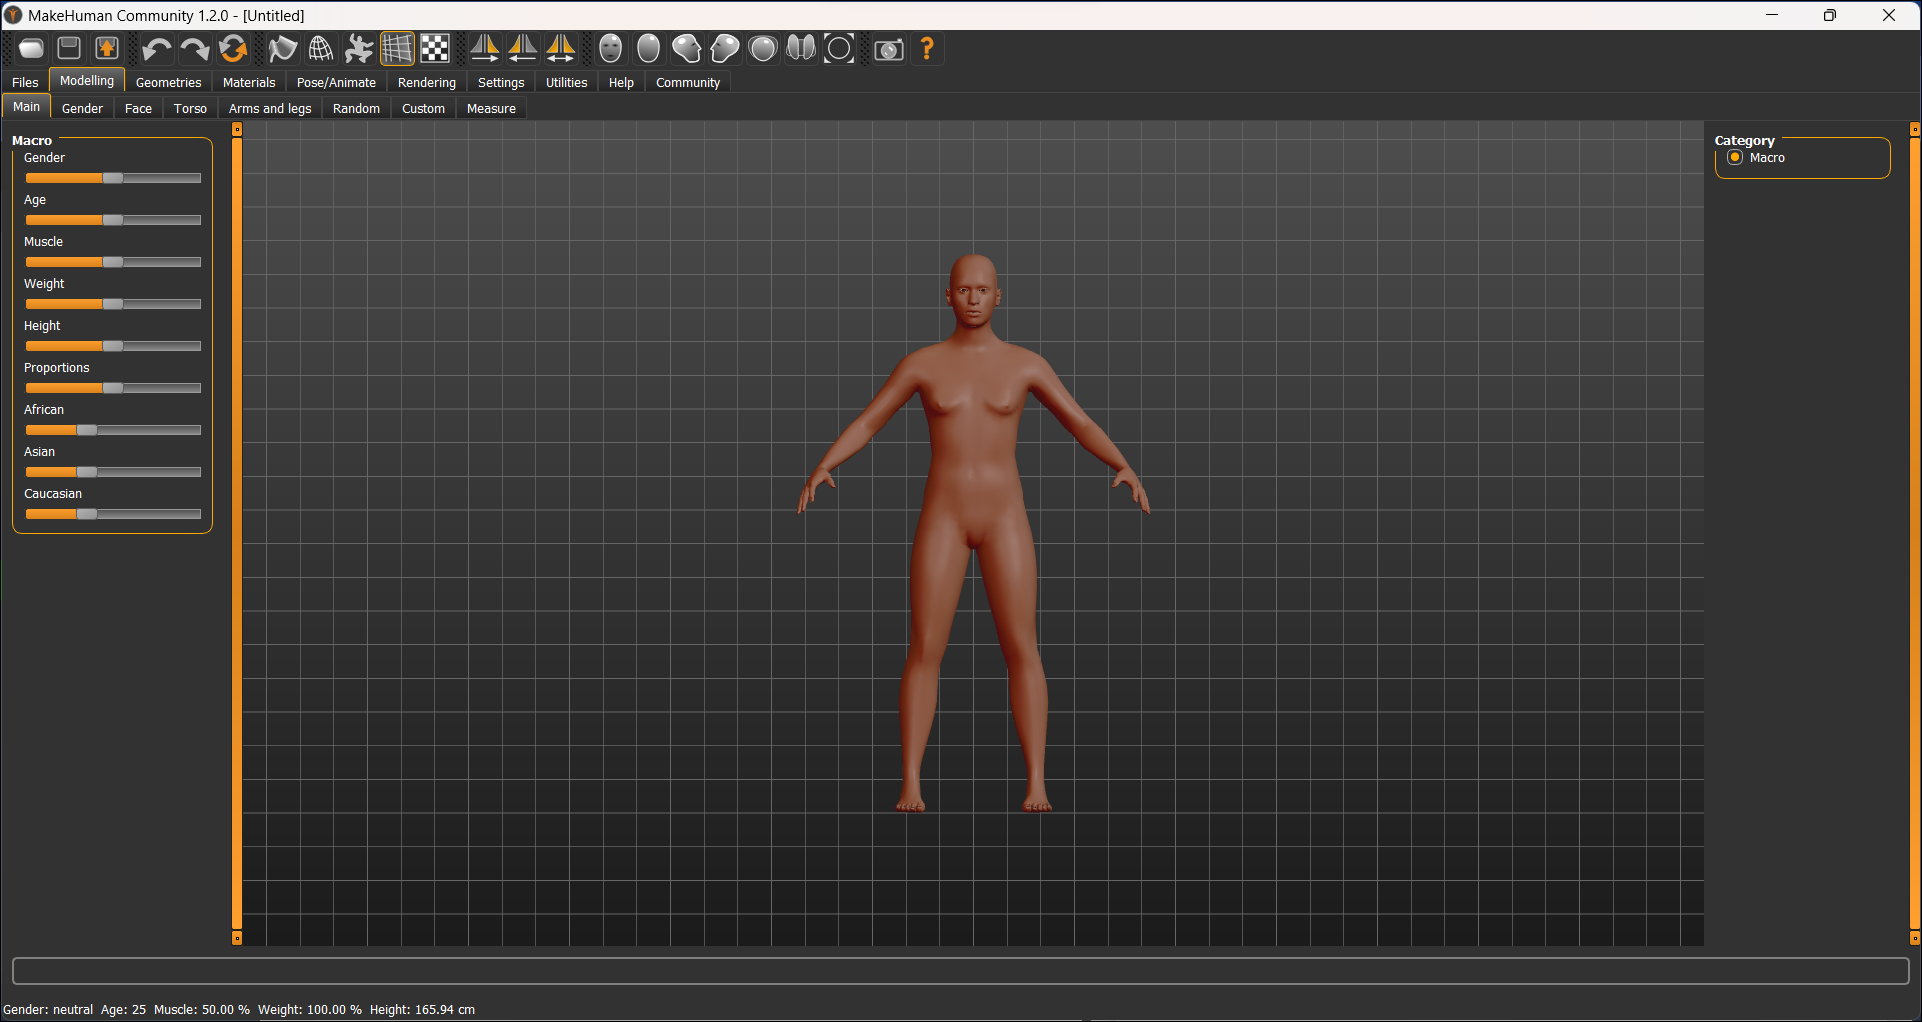
\includegraphics[width=0.9\textwidth]{img/makehuman_landing.png}}
    \caption{Pantalla inicial de \makehuman.}
    \label{fig:makehuman_landing}
    \end{figure}

    \paragraph{}
    En el caso de la aplicación desarrollada, interesaba tener dos modelos 3D distintos, siendo una figura una mujer y otra figura un hombre. Para esto, a través de la primera opción del \textbf{modelado}, \makehuman permite seleccionar conceptos más globales, como el sexo, la edad o la musculatura. A través del resto de categorías dentro de la pestaña principal, la herramienta permite personalizar el resto de secciones del cuerpo, como son la cara, el torso, los brazos y las piernas, cada una de estas con sus propias subcategorías.

    \paragraph{}
    En la pestaña de \textbf{geometrías}, se establecen algunos detalles alternos a las características corporales. Concretamente, se definen formas que van por encima del cuerpo (camisetas, sombreros, pantalones, etc.) o aquellas estructuras corporales que, por su variabilidad, se diseñan paralelamente a este (ojos, pelo, dientes, etc.). En este último caso, a pesar de que \makehuman ofrece muchas opciones, los modelos finalmente utilizados fueron creados con algunos de los recursos generados por la comunidad, concretamente, los ojos, dientes y lengua utilizados. Esta decisión se tomó debido a la necesidad de reducir el peso de la figura todo lo posible para su uso en la web, razón por la cual se optó por escoger recursos de baja resolución para partes del cuerpo que, generalmente, no van a ser visibles o necesitan poco detalle para el uso dado. Estos últimos, sin embargo, no podían omitirse debido a que la figura, al hablar, iba a mostrar tanto lengua como dientes. Para los ojos, por otro lado, se utilizó también una geometría de baja resolución debido a que la diferencia entre esta opción y la de alta resolución no era distinguible en la aplicación de \ra.

    \begin{figure}[H]
    \centering
    \fbox{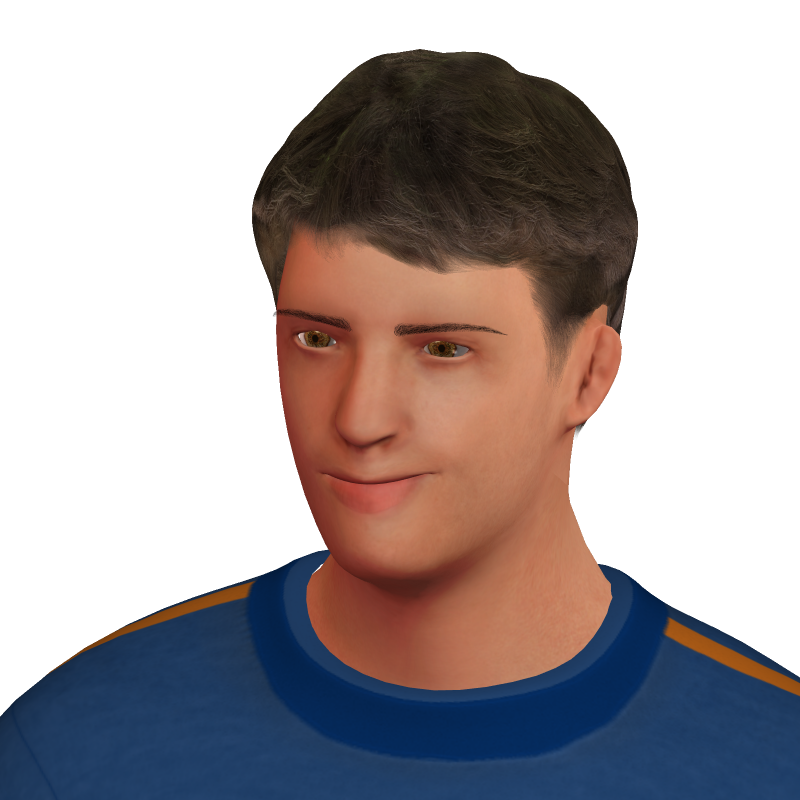
\includegraphics[width=0.6\textwidth]{img/4.1.face_detail.png}}
    \caption{Detalle facial del modelo.}
    \label{fig:4.1.face_detail}
    \end{figure}
    
    \paragraph{}
    Para descargar los recursos que publica la comunidad, existen dos opciones: a través de la web de la aplicación o a través de la propia aplicación, en la pestaña <<\textbf{Community}>>, donde el recurso seleccionado se descargará en la carpeta indicada. Sin embargo, este segundo método es muy lento debido a la propia aplicación, por lo que se optó por descargar los recursos directamente de la web.
    
    \paragraph{}
    Mediante la pestaña de selección de \textbf{materiales}, previa elección de ropa de los modelos en la anterior pestaña, se retocaron dos elementos: la piel del modelo, donde usamos una de las opciones que venían en la aplicación evitando así la piel seleccionada por defecto ya que resulta poco natural; y la textura de la ropa del modelo, donde utilizamos una opción personalizada por nosotros. Para este último, se modificó la propia textura original de la ropa que se seleccionó en la aplicación, siendo este un archivo en formato .png que se puede modificar fácilmente mediante aplicaciones como \textit{GIMP}. En esta modificación probamos varios colores para la camiseta e introdujimos el logotipo de la empresa para darle un aire más <<corporativo>>.

    \begin{figure}[H]
    \centering
    \fbox{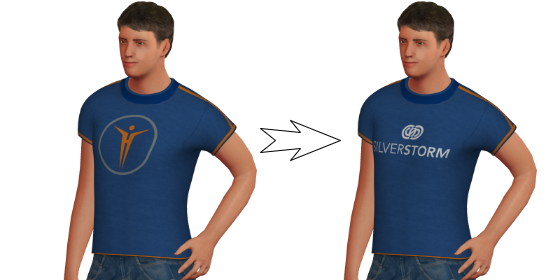
\includegraphics[width=0.5\textwidth]{img/4.1.tshirt_change.png}}
    \caption{Modificación de la textura de la ropa del modelo.}
    \label{fig:4.1.tshirt_change}
    \end{figure}
    
    \paragraph{}
    Finalmente, a través de \textbf{Pose/Animación}, se establece el elemento principal para la posterior animación a través de \blender: el esqueleto. \makehuman ofrece cuatro opciones distintas de esqueletos, donde cada una de estas opciones tiene más o menos huesos, dependiendo del uso que se le quiera dar. Las opciones más básicas controlan únicamente las extremidades, siendo un esqueleto que podría ser útil para animaciones muy básicas. Sin embargo, en este caso, queremos controlas tanto extremidades como músculos faciales, y para este caso, existen dos opciones de esqueletos: <<\textit{Default}>> y <<\textit{Default no toes}>>. Dado que la última opción descarta una serie de huesos que no se van a utilizar en la animación de nuestra aplicación, será la opción que escogeremos, puesto que es algo más ligera.

    \begin{figure}[H]
    \centering
    \fbox{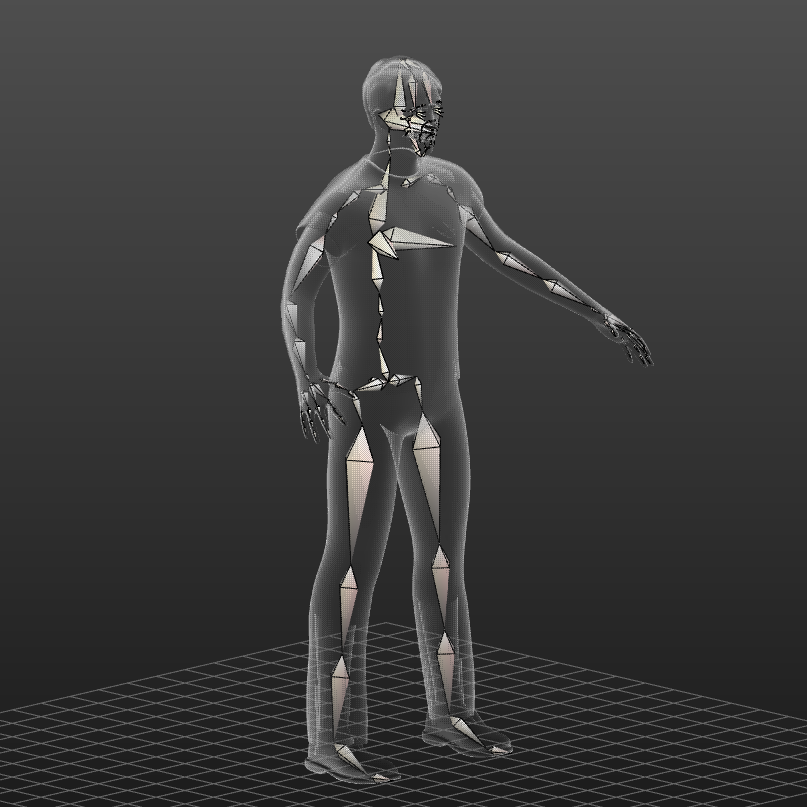
\includegraphics[width=0.6\textwidth]{img/4.1.bones.png}}
    \caption{Detalle de los huesos del modelo.}
    \label{fig:4.1.bones}
    \end{figure}
    
    \paragraph{}
    Para finalizar, en esta última pestaña se le establece también al modelo una posición de reposo y una expresión facial que ofrezcan al personaje una cierta naturalidad, terminando así el diseño del modelo y el trabajo con \makehuman.
    
    \begin{figure}[H]
    \centering
    \fbox{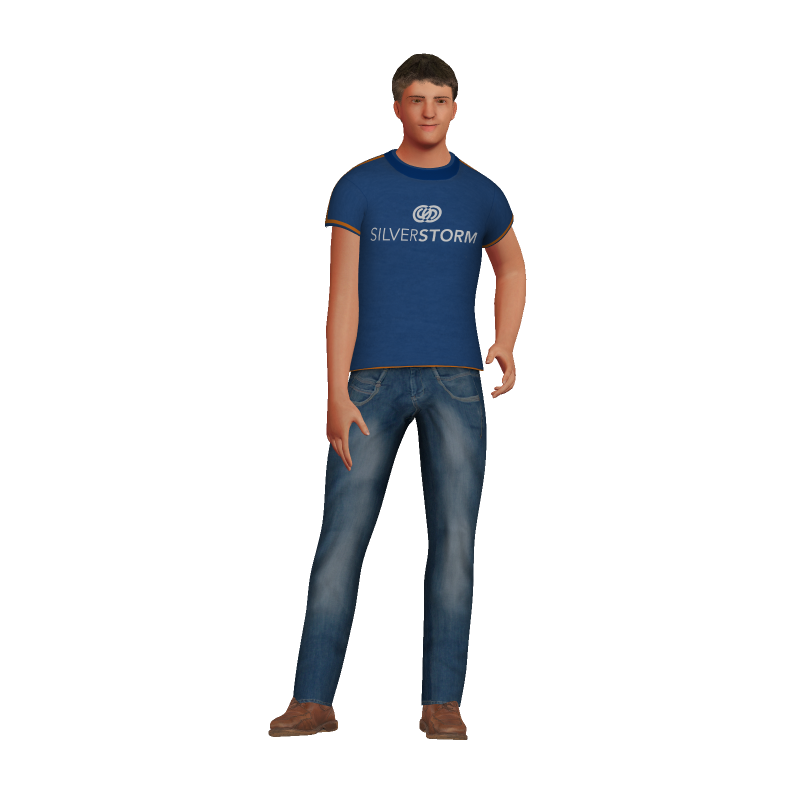
\includegraphics[width=0.6\textwidth]{img/4.1.model_pose.png}}
    \caption{Pose escogida para el modelo.}
    \label{fig:4.1.model_pose}
    \end{figure}
    
    \section{Edición con \blender}
    \label{sec:4.2}

    Para poder continuar el trabajo en \blender, primero es necesario exportar desde \makehuman el trabajo anterior a un formato que puedan entender ambas aplicaciones. \makehuman permite exportar en los formatos \textit{Collada}, \textit{Filmbox}, \textit{MakeHuman Exchange}, \textit{Wavefront obj}, \textit{Ogre3D} y \textit{Estereolitografía}, de los cuales \blender solo es capaz de utilizar tres para la importación sin usar plugins: \textit{Collada}, \textit{Wavefront obj} y \textit{Estereolitografía}. Después de algunas pruebas, se llegó a la conclusión de que el mejor formato para este intercambio entre aplicaciones sería \textit{Collada}, ya que parecía tener menos errores gráficos y mantener la mayor información posible en huesos y posición de la figura. Una vez se ha exportado la figura, solo es necesario importarlo en \blender usando la opción para importar archivos \textit{Collada} en Blender.

    \subsection{Errores gráficos}
    \label{sec:4.2.1}
    Una vez la figura se encuentra preparada para ser modificada en la nueva herramienta, se puede comenzar con las ediciones de errores gráficos. En el momento de importación, se detectaron dos errores en el modelo: por un lado, la textura del pelo, al reducirse la calidad en la exportación, perdía también forma y quedaba <<separado>> de la cabeza; por otro lado, \makehuman prepara el modelo para que aquellas texturas que queden ocultas por diferentes superficies del mismo modelo se borren para ahorrar espacio, siendo sustituidas por texturas transparentes o <<\textit{alpha}>>, pero al modificarse la forma, algunas de estas texturas transparentes quedaban al descubierto, pudiéndose ver lo que había por dentro y por detrás del modelo a través de las transparencias generadas.

    \paragraph{}
    Para el error de forma en el pelo, la solución pasó por un remodelaje manual, utilizando las propias herramientas de modelaje que ofrece \blender. Principalmente se usaron 3 opciones de modelaje: \textit{draw sharp}, \textit{clay thumb} y \textit{crease}, tres formas distintas de incidir la forma del modelo, cada uno de una manera más o menos perfilada. Estas opciones se ocupan de modificar la malla de aristas del modelo, <<aplastándolas>> o desplazándolas según la opción elegida.

    \paragraph{}
    En cuanto al error gráfico de texturas transparentes, la resolución pasó por configurar los canales \textit{alpha} de los materiales, debido a que la configuración utilizada por \makehuman no es la misma que la que utilizan el resto de procesadores de modelos 3D. Para esto, a través del menú \textit{Layout}, se debe seleccionar la opción \textit{Material Properties} para poder modificar las propiedades \textit{Blend Mode} y \textit{Shadow Mode}, a los que se les asignará el valor \textit{Alpha Hashed}. De esta manera, las texturas \textit{alpha} serán interpretadas correctamente y el pelo se verá <<pegado>> a la cabeza

    \subsection{Animaciones}
    \label{sec:4.2.2}
    Después de solucionar los errores gráficos, se puede comenzar con las animaciones del modelo. Estas se dividen en la animación facial y la animación corporal.

    \paragraph{}
    Para esta sección, se utilizará mucho el término <<postura>>, tanto para el modelo como para <<huesos>> del modelo. Es necesario entender dos cosas:
    \begin{itemize}
        \item El hueso, en modelado 3D, es el objeto que, al moverse, desplaza consigo un conjunto de aristas de la textura del modelo
        \item La postura del modelo es la forma en que está dispuesto el conjunto de sus huesos. De la misma manera, la postura de un hueso será cómo estará colocado este en relación a los huesos a los que está unido, teniendo en cuenta principalmente su posición y ángulo.
    \end{itemize}

    \paragraph{}
    Para la animación facial, se añadió un plugin a \blender llamado \rhubarb \cite{web:rhubarb} dedicado a la sincronización labial con audios. Esto se hizo a través de la opción \textit{Add-ons} en el menú de preferencias, donde se da la opción de buscar el plugin y las opciones de instalación, aspecto muy importante ya que la configuración predeterminada está planteada para sincronización labial con textos en inglés.

    \paragraph{}
    Para poder generar la sincronización labial mediante \rhubarb, es necesario hacer uso de las <<librerías de posturas>>: \blender permite almacenar posturas de un modelo para su posterior uso junto con un nombre para estos, de manera que pueden ser utilizados más tarde para diferentes usos. \rhubarb aprovecha esto para que el usuario almacene las formas que adquirirá la boca del modelo al pronunciar algunos de los fonemas más frecuentes, descritos estos en su documentación \cite{web:rhubarb_mouthshapes}. Una vez hecho esto, a través de las herramientas facilitadas por el plugin, se debe asociar cada postura creada con cada conjunto de fonemas mencionado en la documentación.

    \paragraph{}
    Finalizado el primer paso, lo siguiente consiste en proporcionarle al plugin tanto el audio que <<pronunciará>> el modelo como el texto que contiene el diálogo del mismo audio. Después de esto, el plugin generará la animación completa para todo el diálogo, dando un resultado muy fidedigno. En caso de que las animaciones faciales se encuentren a destiempo o no resulten fidedignas, se pueden hacer ajustes a través de las propias herramientas de \blender.

    \begin{figure}%[H]
    \centering
    \fbox{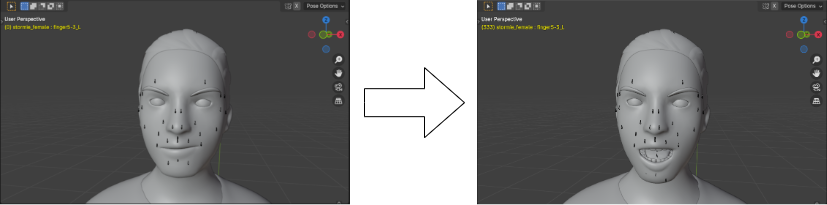
\includegraphics[width=0.95\textwidth]{img/4.2.2_rhubarb.png}}
    \caption{Animación generada a través de \rhubarb.}
    \label{fig:4.2.2_rhubarb}
    \end{figure}

    \paragraph{}
    Por último, se generaron ciertas animaciones corporales para dotar de cierta expresividad y dinamismo al modelo. Puesto que generar animaciones muy realistas es un trabajo muy costoso, se decidió aplicar el conocimiento adquirido para utilizar la herramienta \rhubarb y aplicar el uso de librerías de posturas en la generación de animaciones corporales.

    \paragraph{}
    La ventaja de las posturas grabadas en la librería de posturas es que estas posturas se pueden guardar sobre una serie de huesos del modelo y, después, se puede aplicar sobre los mismos huesos o sobre un subconjunto de los huesos del conjunto original. Esto significa que si, por ejemplo, se ha guardado una postura de un brazo completo (desde el hombro hasta los dedos), después esta misma postura se puede volver a aplicar sobre el brazo completo o solo sobre los dedos. Esto permite generar una serie de posturas y explotarlas a la hora de generar animaciones.

    \paragraph{}
    Una vez se han conseguido una serie de poses válidas, se puede comenzar con la animación. Esto se hace estableciendo la postura que va a tener un hueso en un momento concreto (si no se especifica nada en ningún momento, el hueso va a permanecer en la misma postura hasta el final). Una vez insertado en la animación mediante la opción \textit{Insert keyframe}, el mismo \blender rellena los fotogramas intermedios entre dos posturas distintas con las posturas que adoptará la figura entre una posición y otra para generar la sensación de continuidad y fluidez.

    \begin{figure}%[H]
    \centering
    \fbox{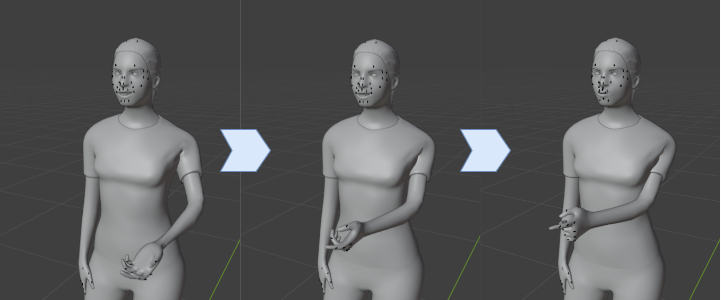
\includegraphics[width=0.9\textwidth]{img/4.2.2_pose_transition.png}}
    \caption{Entre dos posturas grabadas (primera y tercera) se generan posturas intermedias (segunda).}
    \label{fig:4.2.2_pose_transition}
    \end{figure}

    \paragraph{}
    Con las animaciones ya terminadas, finalmente se puede exportar para poder ser utilizado en la aplicación. Para esto, basta con pulsar sobre \textit{File}, \textit{Export} y utilizar la opción \textit{glTF 2.0}. Aquí, nos aseguraremos de que se exporta todo en un solo archivo seleccionando el formato \textit{glTF Binary (.glb)}. Una vez contamos con el archivo, se puede ubicar en el servidor en el destino indicado para los modelos 3D.

\end{document}